虽然多配置、编译器和平台上构建软件是CMake的优势,但这也是其最大的弱点,因为这通常使开发者很难确定哪些构建设置进行过测试,并且适用于给定的软件。3.19版本起,CMake有了预设的特性,可以以可靠和方便的方式处理这些场景。以前,开发人员必须依靠文档和约定来确定CMake项目的首选配置。预设可以指定构建目录、要使用的生成器、目标架构、工具链、缓存变量和要与项目一起使用的环境变量。从CMake 3.20开始,就有了影响构建和测试阶段的预设。

为了使用预设,项目的顶层目录必须包含名为CMakePresets.json或CMakeUserPresets.json的文件。若两个文件都存在,将先解析CMakePresets.json,再解析CMakeUserPresets.json。这两个文件有相同的格式,但使用方式略有不同:

\begin{itemize}
\item 
CMakePresets.json由项目本身提供,并处理项目特定的事情,比如运行CI构建,或若项目本身需要哪些工具链,应该使用哪些工具链进行交叉编译。CMakePresets.json用于特定的项目,不应该引用项目结构外的文件或路径。由于这些预设与项目紧密相连,通常也处于版本控制中。

\item 
CMakeUserPresets.json通常由开发人员定义,以便在自己的机器或构建环境中使用。CMakeUserPresets.json可以尽可能的具体,包含项目之外的路径或特定系统设置特有的路径。因此,项目不应提供此文件,也不应将其置于版本控制中。
\end{itemize}

预设是将缓存变量、编译器标志等移出CMakeLists.txt文件的好方法,同时以一种可以在CMake中使用的方式保持可用的信息,从而提高项目的可移植性。若预置可用,通过命令cmake -{}-listpresets可以从源目录中列出预设:

\begin{tcblisting}{commandshell={}}
Available configure presets:

  "ninja-debug" - Ninja (Debug)
  "ninja-release" - Ninja (Release)
\end{tcblisting}

若设置了displayName属性,预设的名称以带引号的形式列出。在命令行选择预设时,名称需要带引号。

CMake GUI将在源目录中显示所有可用的预设:

\begin{center}
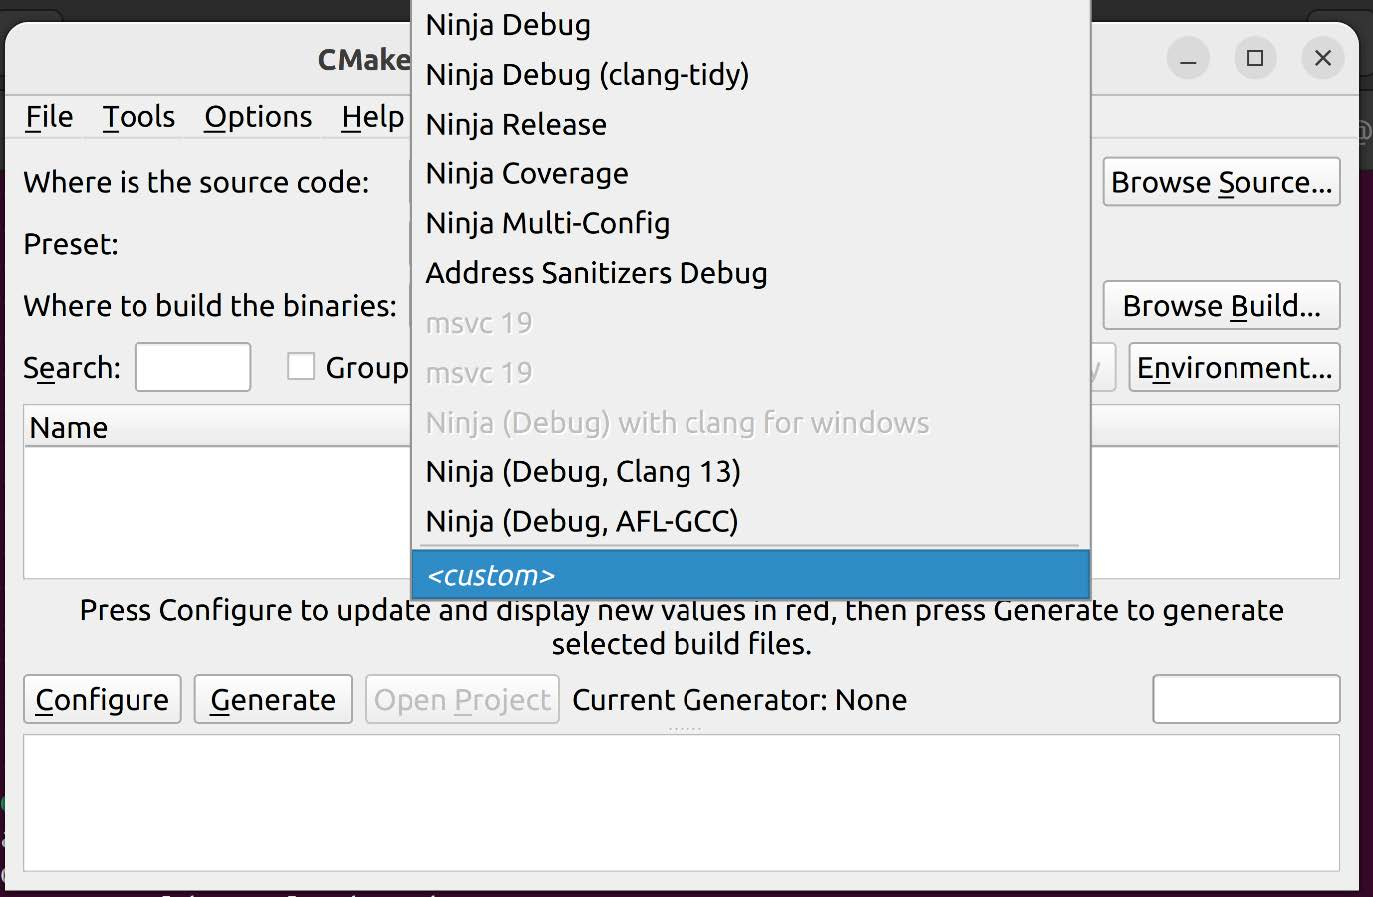
\includegraphics[width=0.8\textwidth]{content/2/chapter9/images/2.jpg}\\
图9.1 CMake GUI中列出可用的预设
\end{center}

CMake的3.21版本,ccmake命令行配置工具不支持预设。需要通过以下命令使用预设,可以从顶层目录中选择配置预设:

\begin{tcblisting}{commandshell={}}
cmake --preset=name
\end{tcblisting}

CMakePresets.json和CMakeUserPresets.json的整体结构是这样的:

\begin{lstlisting}[style=styleCMake]
{
	"version": 3,
	"cmakeMinimumRequired": {"major": 3,"minor": 21,"patch":
		0 },
	"configurePresets": [...],
	"buildPresets": [...],
	"testPresets": [...],
	"vendor": {
		"microsoft.com/VisualStudioSettings/CMake/1.9":
		{ "intelliSenseMode": "windows-msvc-x64"
	} }
}
\end{lstlisting}

version字段指定要使用的JSON模式。版本1是CMake 3.19的第一个版本,只支持configurePresets。版本2增加了buildPresets和testPresets,CMake 3.20开始支持;版本3增加了更多选项,CMake 3.21开始支持。

可选的cmakeMinimumRequired字段可以用来定义构建此项目所需的CMake的最小版本。由于最低要求通常也在CMakeLists.txt文件中说明,这通常会省略。

这三个列表:configurePresets、buildPresets和testPresets,每个列表都包含了用于配置、构建和测试项目的配置。构建和测试的预置要求至少有一个配置预置,将在本节后面看到。

vendor字段包含特定于供应商或IDE信息的可选映射。CMake不解释该字段的内容,除非验证JSON格式。映射的键应该是由斜线分隔的特定于供应商。前面的示例中,供应商预置的键是microsoft.com/VisualStudioSettings/CMake/1.9。供应商字段中的值可以是任何有效的JSON格式。

要使用预置,至少有一个配置预置,定义了CMake配置生成系统的环境。至少应该指定在配置时要使用的构建路径和生成器。配置预设还可为单配置生成器设置常用的缓存变量,如CMAKE\_BUILD\_TYPE。包含配置预设的预设,在Debug模式下用Ninja生成器构建:

\begin{lstlisting}[style=styleCMake]
{
	"version": 3,
	"configurePresets": [
	{
		"name": "ninja",
		"displayName": "Ninja Debug",
		"description": "build in debug mode using Ninja	generator",
		"generator": "Ninja",
		"binaryDir": "build",
		"cacheVariables": { "CMAKE_BUILD_TYPE": "Debug" }
	}
	]
}
\end{lstlisting}

所有预设都必须在预设块内有唯一的名称。由于一些GUI应用程序只显示分配了displayName字段的预设值,因此强烈建议设置这个字段。

\begin{tcolorbox}[colback=blue!5!white,colframe=blue!75!black,title=预设的命名约定]
CMakePresets.json中命名由项目定义的预设是一个很好的方式,以一种不与开发人员在CMakeUserPresets.json中定义名称冲突的方式。常见的约定是在项目定义的预设前加上ci-,以标记其为CI环境所设置。
\end{tcolorbox}

预置的版本1和2中,binaryDir和generator字段是强制的;版本3中,变成了可选的。若没有设置任何字段,其行为与不设置预设的行为相同。CMake的命令行选项将覆盖在预置中的相关值。因此,若设置了binaryDir,则会在调用cmake -{}-preset=时自动创建(-B选项传递的值将覆盖预设中的值)。

缓存变量既可以定义为“键:值”对,如前面的例子所示,也可以定义为JSON对象,这允许指定变量类型。文件路径可以这样指定:

\begin{lstlisting}[style=styleCMake]
"cacheVariables": {
	"CMAKE_TOOLCHAIN_FILE": {
		"type": "FILEPATH",
		"value": "${sourceDir}/cmake/toolchain.cmake"
	}
}
\end{lstlisting}

若使用key:value形式,该类型将视为STRING,除非是true或false(没有引号),将解释为BOOL。注意示例中的\$\{sourceDir\},这个宏在使用预设时展开。

以下是一些常用宏:

\begin{itemize}
\item 
\$\{sourceDir\}: 指向项目源目录,\$\{sourceParentDir\}指向源目录的父目录。不带源目录路径的目录名可以通过\$\{sourceDirName\}获得。若\$\{sourceDir\}是/home/sandy/MyProject,\$\{sourceDirName\}将是MyProject, \$\{sourceParentDir\}将是/home/sandy/。

\item 
\$\{generator\}: 这包含由所使用的当前预设指定的生成器。对于构建和测试预设,包含配置预设的生成器。

\item 
\$\{hostSystemName\}: 主机操作系统的系统名称,与CMAKE\_HOST\_SYSTEM相同。该值可以是uname -s或Linux、Windows或Darwin(用于macOS)的结果。

\item
\$env\{<variable-name>\}: 包含名为<variable-name>的环境变量。若在预置中使用环境字段定义变量,则使用此值。使用\$penv\{<variable-name>\}的工作原理类似,即使它定义了,该值也取自父环境,这允许在现有的环境变量中增加值。因为其不允许循环引用,所以不能使用\$env\{…\}。注意,在Windows环境中,变量是不区分大小写的;在预设中使用的变量区分大小写。因此,建议与环境变量的Shell环境保持一致。

\item
\$vendor\{<macro-name>\}: 这是IDE供应商插入自己宏的扩展点。由于CMake不能解释这些宏,使用\$vendor\{…\}宏的预设将会忽略。

\item
\$\{dollar\}: 这是字面美元符号\$的占位符。
\end{itemize}

修改预置环境的工作原理类似于设置缓存变量:通过设置环境字段,该字段包含“键:值”对的映射。即使值为空,也始终设置环境变量。环境变量可以相互引用,只要不包含循环引用:

\begin{lstlisting}[style=styleCMake]
{
	"version": 3,
	"configurePresets": [
	{
		"name": "ci-ninja",
		"generator": "Ninja",
		"binaryDir": "build",
		"environment": {
			"PATH": "${sourceDir}/scripts:$penv{PATH}",
			"LOCAL_PATH": "$env{PATH}",
			"EMPTY" : null
		}
	}
	]
}
\end{lstlisting}

本例中,PATH环境变量通过从项目结构中来添加路径,使用\$penv\{PATH\}宏可以确保该值来自预设值外,然后LOCAL\_PATH变量通过使用\$env\{PATH\}宏引用修改过的PATH环境变量。只要PATH环境变量不包含会创建循环引用的\$env\{LOCAL\_PATH\},这个引用就没问题。通过传递null来取消设置EMPTY环境变量。注意,null没有加引号。除非使用构建预设或测试预设,否则环境不会转发至相应的步骤。若使用了构建或测试预设,但不应用来自配置预设的环境,则可以在将inheritConfigureEnvironment字段设置为false,显式地进行声明。

\subsubsubsection{9.2.1\hspace{0.2cm}继承预设}

预置可以从与inherited字段的相同类型的其他预置继承,该字段可以包含单个预置或预置列表。从父字段继承字段时,可以覆盖预置或添加其他字段。这有助于避免通用构建块的代码重复。结合隐藏字段,这可以减少CMakePreset.json文件的大小。考虑下面的例子:

\begin{lstlisting}[style=styleCMake]
{
	"version": 3,
	"configurePresets": [
	{
		"name": "ci-ninja",
		"generator": "Ninja",
		"hidden": true,
		"binaryDir": "build"
	},
	{
		"name": "ci-ninja-debug",
		"inherits": "ci-ninja",
		"cacheVariables": {
			"CMAKE_BUILD_TYPE": "Debug"
		}
	},
	{
		"name": "ci-ninja-release",
		"inherits": "ci-ninja",
		"cacheVariables": {
			"CMAKE_BUILD_TYPE": "Release"
		}
	}
	]
}
\end{lstlisting}

本例中,ci-ninja-debug和ci-ninja-release预置都继承自隐藏的ci-ninja构建预置,并将CMAKE\_BUILD\_TYPE缓存变量设置为各自的配置。仍然可以使用隐藏的预设,但在调用cmake -{}-list-presets时不会显示。CMakeUserPreset.json中定义的预设可能继承自CMakePreset.json。

前面的例子中,预设从一个父级继承,但也可以从多个父级继承。下面的例子展示了CMakeUserPreset.json如何与前面例子中的CMakePreset.json一起工作:

\begin{lstlisting}[style=styleCMake]
{
	"version": 3,
	"configurePresets": [
	{
		"name": "gcc-11",
		"hidden": true,
		"binaryDir": "build",
		"cacheVariables": {
			"CMAKE_C_COMPILER": "gcc-11",
			"CMAKE_CXX_COMPILER": "g++-11"
		}
	},
	{
		"name": "ninja-debug-gcc",
		"inherits": ["ci-ninja-debug","gcc-11"]
	},
	]
}
\end{lstlisting}

用户提供了一个预设,它显式选择GCC 11作为名为gcc-11的编译器。之后,ninja-debug-gcc预设从CMakePreset.json中定义的ninja-debug预设继承值,并将其与用户提供的gcc-11预置相结合。若两个父预设为同一字段定义不同的值,则继承列表中第一个出现的值优先。

\subsubsubsection{9.2.2\hspace{0.2cm}预设的条件}

有时预设只在特定的条件下才有意义,例如:对于特定的构建平台。使用Visual Studio生成器的配置预设只在Windows环境中有用,若条件选项不满足条件,则可以禁用预设。继承父预设中定义的条件。条件可以是常量、字符串比较或检查列表是否包含值,可以从预设的版本3中获得。以下配置预设只会在Windows上启用:

\begin{lstlisting}[style=styleCMake]
{
	"name": "ci-msvc-19",
	"generator": "Visual Studio 16 2019",
	"binaryDir": "build",
	"condition": {
		"type": "equals",
		"lhs": "${hostSystemName}",
		"rhs": "Windows"
	}
}
\end{lstlisting}

前面的示例中,若使用\$\{hostSystemName\}宏检索主机系统的名称,然后将其与Windows字符串进行比较,则构建预设是启用的。若\$\{hostSystemName\}匹配,则启用预设,否则禁用预设,尝试使用它将导致错误。比较字符串时,大小写很重要:对于不区分大小写的测试,可以使用接受正则表达式的matches或notMatches类型。

对于更复杂的条件,支持使用allOf、anyOf和not操作符的布尔逻辑嵌套。若配置预置只在Windows和Linux中启用,而在macOS中不启用,则预置和条件可以如下所示:

\begin{lstlisting}[style=styleCMake]
{
	"name": "WindowsAndLinuxOnly",
	"condition": {
		"type": "anyOf",
		"conditions": [
		{
			"type": "equals",
			"lhs": "${hostSystemName}",
			"rhs": "Windows"
		},
		{
			"type": "equals",
			"lhs": "${hostSystemName}",
			"rhs": "Linux"
		}
		]
	}
\end{lstlisting}

每个条件还可以包含更多的嵌套条件,尽管这样做会增加预设的复杂性。

目前,我们只在示例中看到了配置预置,还有构建预置和测试预置。构建和测试预置的语法非常类似于配置预置和许多字段,如name、displayName和inherit,条件的工作原理与配置预置相同。

生成预设必须在configure预设字段中指定一个配置预设,或者从指定配置预设的另一个生成预设继承。构建目录由配置预设确定,并且继承来自配置预设的环境,除非将inheritConfigureEnvironment字段设置为false。构建预设可以指定要构建的目标列表:

\begin{lstlisting}[style=styleCMake]
{
	"version": 3,
	"configurePresets": [
	{
		"name": "ci-msvc-19",
		"displayName": "msvc 19",
		"description": "Configuring for msvc 19",
		"generator": "Visual Studio 16 2019",
		"binaryDir" : "build"
	}
	],
	"buildPresets": [
	{
		"name": "ci-msvc-debug",
		"configurePreset": "ci-msvc-19",
		"configuration": "Debug"
	},
	{
		"name": "ci-msvc-release",
		"configurePreset": "ci-msvc-19",
		"configuration": "Release"
	},
	{
		"name": "ci-documentation",
		"configurePreset": "ci-msvc-19",
		"targets": [
		"api-doc",
		"doc"
		]
	}
	]
}
\end{lstlisting}

示例中,定义了三个构建预置。其中两个用于指定Visual Studio的构建配置,第三个列出了作为文档构建的一部分的api-doc和文档目标。调用ci-msvc构建预设将构建“all”目标,而ci-documentation将只构建列出的目标。可用的构建预设列表可以用cmake -{}-build -{}-list-presets来检索。

测试预设的工作原理与构建预设相似,不同的是它们与CTest一起使用。类似地,在项目根目录上调用ctest -{}-list-presets将列出可用的测试预置。测试预设可用于选择或排除某些测试、指定固件选项或控制测试的输出,测试预设的例子:

\begin{lstlisting}[style=styleCMake]
{
	"version": 3,
	"configurePresets": [
	{
		"name": "ci-ninja",
		...
	}
	"testPresets": [
	{
		"name": "ci-feature-X",
		"configurePreset": "ci-ninja",
		"filter": {
			"include": {
				"name": "feature-X"
			},
			"exclude": {
				"label": "integration"
			}
		}
	}
	]
}
\end{lstlisting}

前面的示例中,添加了一个测试预置,过滤包含feature-X测试,排除标记为integration的测试。这相当于在构建目录下使用以下命令:

\begin{tcblisting}{commandshell={}}
ctest --tests-regex feature-X --label-exclude integration
\end{tcblisting}

自引入目标以来,CMake预设可以说是少数几个改变CMake使用方式的特性。它们是一个折衷方案,可以在交付公共配置和与项目一起构建选项的同时,仍然保持CMakeLists.txt文件与平台无关。然而,有时提供必要的设置是不够的,还会希望共享一个构建环境,在该环境中可以确定软件可以编译。一种选择是定义一个包含CMake和必要库的容器。















